\section{Autoencoders}
\begin{frame}{What is an Autoencoder?}

\textbf{Autoencoder:} a type of neural network that learn to compress data into a compact form and then reconstruct it to match the original input.

% \hspace{0.2em}

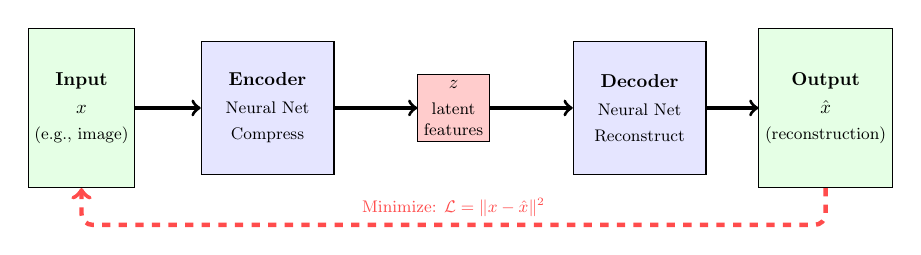
\begin{tikzpicture}[scale=0.675, transform shape]
     % Input
     \node[draw, rectangle, fill=green!10, minimum width=2cm, minimum height=3cm, align=center] (input) at (0,0) {
         \textbf{Input}\\[0.3em]
         $x$\\[0.2em]
         \small (e.g., image)
     };

     % Encoder
     \node[draw, rectangle, fill=blue!10, minimum width=2.5cm, minimum height=2.5cm, align=center] (encoder) at (3.5,0) {
         \textbf{Encoder}\\[0.3em]
         \small Neural Net\\[0.2em]
         \small Compress
     };

     % Latent/Bottleneck
     \node[draw, rectangle, fill=red!20, minimum width=1.2cm, minimum height=1.2cm, align=center] (latent) at (7,0) {
         \textbf{$z$}\\[0.2em]
         \small latent\\[-0.1em]
         \small features
     };

     % Decoder
     \node[draw, rectangle, fill=blue!10, minimum width=2.5cm, minimum height=2.5cm, align=center] (decoder) at (10.5,0) {
         \textbf{Decoder}\\[0.3em]
         \small Neural Net\\[0.2em]
         \small Reconstruct
     };

     % Output
     \node[draw, rectangle, fill=green!10, minimum width=2cm, minimum height=3cm, align=center] (output) at (14,0) {
         \textbf{Output}\\[0.3em]
         $\hat{x}$\\[0.2em]
         \small (reconstruction)
     };

     % Forward arrows
     \draw[->, very thick] (input) -- (encoder);
     \draw[->, very thick] (encoder) -- (latent);
     \draw[->, very thick] (latent) -- (decoder);
     \draw[->, very thick] (decoder) -- (output);

     % Loss arrow (Corrected: Squared path underneath)
     % Goes Down -> Left -> Up
     \draw[->, dashed, red!70, ultra thick, rounded corners] 
        (output.south) -- (14,-2.2) -- node[midway, above, font=\small] {Minimize: $\mathcal{L} = \|x - \hat{x}\|^2$} (0,-2.2) -- (input.south);

\end{tikzpicture}

\vspace{0.5em}
\textbf{The trick:} Force information through a narrow \textbf{bottleneck} $z$.

\vspace{0.2em}
\centering
\small This forces the network to learn compressed, meaningful representations!

\end{frame}

% --- SLIDE 3: Why Does This Work? ---
\begin{frame}{Why Does the Bottleneck Work?}
What if there's no bottleneck?

\vspace{1.5em}
\begin{columns}[c]
\begin{column}{0.48\textwidth}
\textbf{Without Bottleneck}

\vspace{0.3em}
\centering
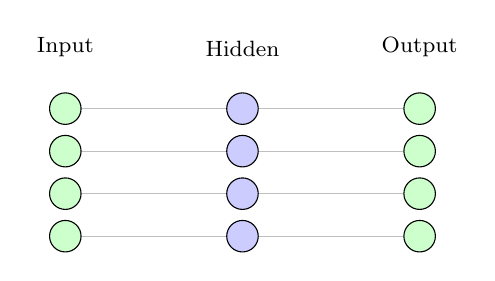
\begin{tikzpicture}[scale=0.9]
    % Input layer
    \foreach \i in {1,...,4} {
        \node[circle, draw, fill=green!20, minimum size=0.4cm] (i\i) at (0, -\i*0.6) {};
    }
    \node[above, font=\footnotesize] at (0, 0) {Input};
    
    % Hidden layer (same size)
    \foreach \i in {1,...,4} {
        \node[circle, draw, fill=blue!20, minimum size=0.4cm] (h\i) at (2.5, -\i*0.6) {};
    }
    \node[above, font=\footnotesize] at (2.5, 0) {Hidden};
    
    % Output layer
    \foreach \i in {1,...,4} {
        \node[circle, draw, fill=green!20, minimum size=0.4cm] (o\i) at (5, -\i*0.6) {};
    }
    \node[above, font=\footnotesize] at (5, 0) {Output};
    
    % Identity connections
    \foreach \i in {1,...,4} {
        \draw[gray!50] (i\i) -- (h\i) -- (o\i);
    }
\end{tikzpicture}

\vspace{0.3em}
\small Network can just copy:\\
$h_i = x_i$, $\hat{x}_i = h_i$

\vspace{0.3em}
{\color{red} Learns nothing useful!}
\end{column}

\begin{column}{0.48\textwidth}
\textbf{With Bottleneck}

\vspace{0.3em}
\centering
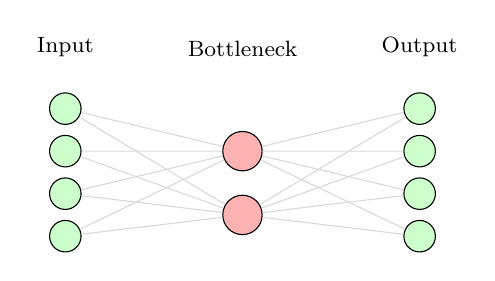
\begin{tikzpicture}[scale=0.9]
    % Input layer
    \foreach \i in {1,...,4} {
        \node[circle, draw, fill=green!20, minimum size=0.4cm] (i\i) at (0, -\i*0.6) {};
    }
    \node[above, font=\footnotesize] at (0, 0) {Input};
    
    % Bottleneck (smaller)
    \foreach \i in {1,2} {
        \node[circle, draw, fill=red!30, minimum size=0.5cm] (b\i) at (2.5, -\i*0.9-0.3) {};
    }
    \node[above, font=\footnotesize] at (2.5, 0) {Bottleneck};
    
    % Output layer
    \foreach \i in {1,...,4} {
        \node[circle, draw, fill=green!20, minimum size=0.4cm] (o\i) at (5, -\i*0.6) {};
    }
    \node[above, font=\footnotesize] at (5, 0) {Output};
    
    % Full connections
    \foreach \i in {1,...,4} {
        \foreach \j in {1,2} {
            \draw[gray!30] (i\i) -- (b\j);
            \draw[gray!30] (b\j) -- (o\i);
        }
    }
\end{tikzpicture}

\vspace{0.3em}
\small Must compress 4D $\rightarrow$ 2D\\
Forces learning of structure!

\vspace{0.3em}
{\color{green!60!black} Learns meaningful features!}
\end{column}
\end{columns}

\end{frame}

% --- SLIDE 7: Application 1 - Dimensionality Reduction ---% --- SLIDE 7: Application 1 - Dimensionality Reduction ---
\begin{frame}{Application 1: Dimensionality Reduction}

\textbf{How to use an Autoencoder for compression:}

\vspace{0.5em}
\centering
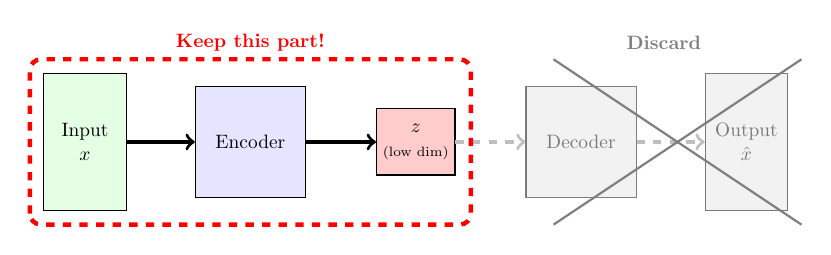
\begin{tikzpicture}[scale=0.7, transform shape]
    % Nodes
    \node[draw, rectangle, fill=green!10, minimum width=1.5cm, minimum height=2.5cm, align=center] (input) at (0,0) {Input\\$x$};
    
    \node[draw, rectangle, fill=blue!10, minimum width=2cm, minimum height=2cm, align=center] (encoder) at (3,0) {Encoder};
    
    \node[draw, rectangle, fill=red!20, minimum width=1.2cm, minimum height=1.2cm, align=center] (latent) at (6,0) {$z$\\\scriptsize(low dim)};
    
    \node[draw, rectangle, fill=gray!20, minimum width=2cm, minimum height=2cm, align=center, opacity=0.5] (decoder) at (9,0) {Decoder};
    
    \node[draw, rectangle, fill=gray!20, minimum width=1.5cm, minimum height=2.5cm, align=center, opacity=0.5] (output) at (12,0) {Output\\$\hat{x}$};
    
    % Arrows
    \draw[->, very thick] (input) -- (encoder);
    \draw[->, very thick] (encoder) -- (latent);
    \draw[->, very thick, gray!50, dashed] (latent) -- (decoder);
    \draw[->, very thick, gray!50, dashed] (decoder) -- (output);
    
    % Highlight Box (The Encoder Part)
    \draw[red, ultra thick, dashed, rounded corners] (-1, -1.5) rectangle (7, 1.5);
    \node[red, font=\bfseries] at (3, 1.8) {Keep this part!};
    
    % Discard label
    \node[gray, font=\bfseries] at (10.5, 1.8) {Discard};
    \draw[thick, gray] (8.5, -1.5) -- (13, 1.5);
    \draw[thick, gray] (8.5, 1.5) -- (13, -1.5);
\end{tikzpicture}

\vspace{1em}
\begin{tcolorbox}[colback=blue!5, colframe=blue!50, title=\textbf{The Process}]
\begin{enumerate}
    \item \textbf{Train} the full network to reconstruct the input ($x \approx \hat{x}$).
    \item \textbf{Discard} the Decoder (it's only needed for training).
    \item \textbf{Use the Encoder} to map high-dimensional data $x$ to low-dimensional code $z$.
\end{enumerate}
\end{tcolorbox}

\end{frame}

% --- SLIDE: Application - Image Generation ---
\begin{frame}{Application 2: Image Generation}

\textbf{How to use an Autoencoder for generation:}

\vspace{0.5em}
\centering
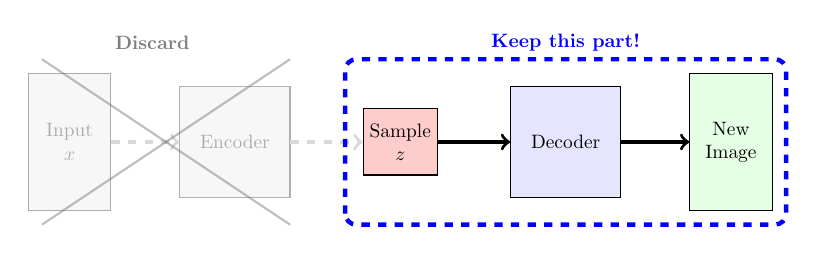
\begin{tikzpicture}[scale=0.7, transform shape]
    % Nodes (Ghosted Encoder side)
    \node[draw, rectangle, fill=gray!20, minimum width=1.5cm, minimum height=2.5cm, align=center, opacity=0.3] (input) at (0,0) {Input\\$x$};
    
    \node[draw, rectangle, fill=gray!20, minimum width=2cm, minimum height=2cm, align=center, opacity=0.3] (encoder) at (3,0) {Encoder};
    
    % Active Latent Code
    \node[draw, rectangle, fill=red!20, minimum width=1.2cm, minimum height=1.2cm, align=center] (latent) at (6,0) {Sample\\$z$};
    
    % Active Decoder side
    \node[draw, rectangle, fill=blue!10, minimum width=2cm, minimum height=2cm, align=center] (decoder) at (9,0) {Decoder};
    
    \node[draw, rectangle, fill=green!10, minimum width=1.5cm, minimum height=2.5cm, align=center] (output) at (12,0) {New\\Image};
    
    % Arrows
    \draw[->, very thick, gray!30, dashed] (input) -- (encoder);
    \draw[->, very thick, gray!30, dashed] (encoder) -- (latent);
    \draw[->, very thick] (latent) -- (decoder);
    \draw[->, very thick] (decoder) -- (output);
    
    % Highlight Box (The Decoder Part)
    \draw[blue, ultra thick, dashed, rounded corners] (5, -1.5) rectangle (13, 1.5);
    \node[blue, font=\bfseries] at (9, 1.8) {Keep this part!};
    
    % Discard label
    \node[gray, font=\bfseries] at (1.5, 1.8) {Discard};
    \draw[thick, gray, opacity=0.5] (-0.5, -1.5) -- (4, 1.5);
    \draw[thick, gray, opacity=0.5] (-0.5, 1.5) -- (4, -1.5);
\end{tikzpicture}

\vspace{1em}
\begin{tcolorbox}[colback=purple!5, colframe=purple!50, title=\textbf{The Process}]
\begin{enumerate}
    \item \textbf{Train} the full network on images to learn features.
    \item \textbf{Discard} the Encoder.
    \item \textbf{Sample} a random vector $z$ (pick random numbers).
    \item \textbf{Generate} a brand new image by running $z$ through the Decoder.
\end{enumerate}
\end{tcolorbox}
\end{frame}
% --- SLIDE: Application - Denoising (Redesigned) ---
\begin{frame}{Application 3: Denoising Autoencoders}

\textbf{Idea:} Train the network to recover the original signal from corrupted input.

\vspace{0.5em}
\centering
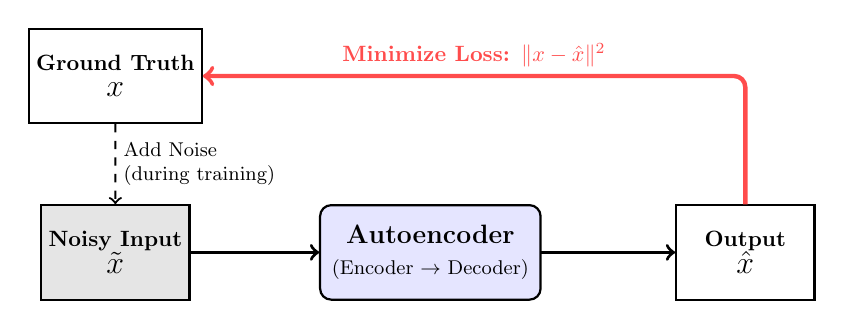
\begin{tikzpicture}[scale=0.8, transform shape]
    % --- Nodes ---
    
    % 1. Ground Truth (Top Left)
    \node[draw, thick, fill=white, minimum width=2.2cm, minimum height=1.5cm, align=center] (clean) at (0, 2.8) {
        \textbf{Ground Truth}\\
        \Large $x$
    };
    
    % 2. Noisy Input (Bottom Left)
    \node[draw, thick, fill=gray!20, minimum width=2.2cm, minimum height=1.5cm, align=center] (noisy) at (0, 0) {
        \textbf{Noisy Input}\\
        \Large $\tilde{x}$
    };
    
    % 3. Autoencoder (Center)
    \node[draw, thick, fill=blue!10, rounded corners, minimum width=3.5cm, minimum height=1.5cm, align=center, font=\large] (ae) at (5, 0) {
        \textbf{Autoencoder}\\
        \small (Encoder $\to$ Decoder)
    };
    
    % 4. Output (Bottom Right)
    \node[draw, thick, fill=white, minimum width=2.2cm, minimum height=1.5cm, align=center] (output) at (10, 0) {
        \textbf{Output}\\
        \Large $\hat{x}$
    };
    
    % --- Arrows ---
    
    % Noise Process (Down)
    \draw[->, thick, dashed] (clean) -- node[midway, right, font=\small, align=left] {Add Noise\\(during training)} (noisy);
    
    % Forward Pass (Right)
    \draw[->, very thick] (noisy) -- (ae);
    \draw[->, very thick] (ae) -- (output);
    
    % Loss Calculation (Up and Left)
    % Connecting Output back to Ground Truth for loss
    \draw[->, red!70, ultra thick, rounded corners] (output.north) -- (10, 2.8) -- node[midway, above, font=\bfseries] {Minimize Loss: $\|x - \hat{x}\|^2$} (clean.east);

\end{tikzpicture}

    \begin{tcolorbox}[colback=yellow!10, colframe=orange!50, title=\textbf{How it works}]
    \begin{itemize}
        \item Take clean image $x$.
        \item Corrupt it to get $\tilde{x}$.
        \item Force AE to map $\tilde{x} \rightarrow x$.
    \end{itemize}
    \end{tcolorbox}


\end{frame}

% --- SLIDE: Application - Anomaly Detection ---
\begin{frame}{Application 4: Anomaly Detection}

\textbf{Concept:} The network learns to reconstruct "Normal" data perfectly. When it sees an anomaly, it fails to reconstruct it.

\vspace{0.5em}
\centering
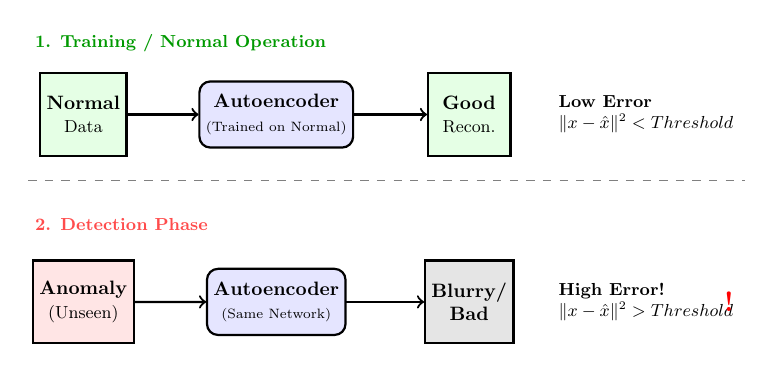
\begin{tikzpicture}[scale=0.7, transform shape]

    % --- SCENARIO 1: NORMAL (Top) ---
    \node[anchor=west, font=\bfseries\small, green!60!black] at (-3, 2.5) {1. Training / Normal Operation};
    
    % Input Normal
    \node[draw, thick, fill=green!10, minimum width=1.5cm, minimum height=1.5cm, align=center] (norm_in) at (-2, 1.2) {
        \textbf{Normal}\\
        \small Data
    };

    % Autoencoder (Shared)
    \node[draw, thick, fill=blue!10, rounded corners, minimum width=2.5cm, minimum height=1.2cm, align=center] (ae_top) at (1.5, 1.2) {
        \textbf{Autoencoder}\\
        \scriptsize (Trained on Normal)
    };

    % Output Normal
    \node[draw, thick, fill=green!10, minimum width=1.5cm, minimum height=1.5cm, align=center] (norm_out) at (5, 1.2) {
        \textbf{Good}\\
        \small Recon.
    };

    % Result
    \node[right, align=left, font=\small] at (6.5, 1.2) {
        \textbf{Low Error}\\
        $\|x - \hat{x}\|^2 < \text{Threshold}$
    };
    \node[right, green!60!black, font=\Large] at (9.5, 1.2) {\checkmark};

    % Arrows
    \draw[->, thick] (norm_in) -- (ae_top);
    \draw[->, thick] (ae_top) -- (norm_out);


    % --- SEPARATOR LINE ---
    \draw[dashed, gray] (-3, 0) -- (10, 0);


    % --- SCENARIO 2: ANOMALY (Bottom) ---
    \node[anchor=west, font=\bfseries\small, red!70] at (-3, -0.8) {2. Detection Phase};

    % Input Anomaly
    \node[draw, thick, fill=red!10, minimum width=1.5cm, minimum height=1.5cm, align=center] (anom_in) at (-2, -2.2) {
        \textbf{Anomaly}\\
        \small (Unseen)
    };

    % Autoencoder (Same one)
    \node[draw, thick, fill=blue!10, rounded corners, minimum width=2.5cm, minimum height=1.2cm, align=center] (ae_bot) at (1.5, -2.2) {
        \textbf{Autoencoder}\\
        \scriptsize (Same Network)
    };

    % Output Poor
    \node[draw, thick, fill=gray!20, minimum width=1.5cm, minimum height=1.5cm, align=center] (anom_out) at (5, -2.2) {
        \textbf{Blurry/}\\
        \textbf{Bad}
    };

    % Result
    \node[right, align=left, font=\small] at (6.5, -2.2) {
        \textbf{High Error!}\\
        $\|x - \hat{x}\|^2 > \text{Threshold}$
    };
    \node[right, red, font=\Large] at (9.5, -2.2) {\textbf{!}};

    % Arrows
    \draw[->, thick] (anom_in) -- (ae_bot);
    \draw[->, thick] (ae_bot) -- (anom_out);

\end{tikzpicture}

% \vspace{0.8em}
\begin{tcolorbox}[colback=yellow!10, colframe=orange!50, title=\textbf{Real-World Use Cases}]
\begin{itemize}
    \item \textbf{Credit Card Fraud:} Normal transactions reconstruct well, theft looks weird.
    \item \textbf{Manufacturing:} Detect defective parts on an assembly line.
\end{itemize}
\end{tcolorbox}

\end{frame}


% --- PART 6: SUMMARY ---
\section{References}
